\documentclass[titlepage,12pt,a4paper]{article}

\usepackage[pdftex]{graphicx}
%\usepackage[symbol]{footmisc}
\usepackage[utf8]{inputenc}

\usepackage{tikz}
\usetikzlibrary{shapes,decorations}

\usepackage{makeidx}
%\usepackage{showidx}
\usepackage{parskip}
\usepackage{float}
\usepackage{calc}
\usepackage{pdfpages}
\usepackage{todonotes}
\usepackage{amsfonts}
\usepackage{amsmath}
\usepackage{pifont}
\usepackage{pdflscape}
\usepackage{geometry}

\usepackage[backref=page]{hyperref}
\def\backref#1{{\scriptsize [#1]}}

\newcommand{\HRule}{\rule{\linewidth}{0.35mm}}

\def\theaipage{\string\hyperpage{\thepage}}

\hypersetup{
    %bookmarks=true,         % show bookmarks bar?
    unicode=false,          % non-Latin characters in Acrobats bookmarks
    pdftoolbar=true,        % show Acrobats toolbar?
    pdfmenubar=true,        % show Acrobats menu?T
    pdffitwindow=false,     % window fit to page when opened
    pdfstartview={FitH},    % fits the width of the page to the window
    pdftitle={Design of Liaison System, TFE4140 Term Project},    % title
    pdfauthor={Stian Hvatum, Benjamin Bjørnseth},     % author
    pdfsubject={TFE4140 Term Project},   % subject of the document
    pdfcreator={Stian Hvatum, Benjamin Bjørnseth},   % creator of the document
    pdfproducer={Stian Hvatum, Benjamin Bjørnseth}, % producer of the document
    pdfnewwindow=true,      % links in new window
    colorlinks,       % false: boxed links; true: colored links
    linkcolor=black,          % color of internal links
    citecolor=green,        % color of links to bibliography
    filecolor=magenta,      % color of file links
    urlcolor=cyan           % color of external links
}

\begin{document}

\begin{titlepage}

\begin{center}

    %    \includegraphics[scale=0.7]{./figures/Fortitudo_floris}\\[1cm]

\textsc{\LARGE TTK4850 - EiT Byggelandsbyen}\\[0.2cm]

\HRule \\[0.5cm]

{\huge Miksebord}\\[0.2cm]
\small{Project report}\\[1cm]

\begin{table}[h]
\centering
\begin{tabular}{rl}
Thomas Hasfjord   &  Bård Bakken Stovner\\
Andreas Eilertsen & Håkon Furre Amundsen\\
\multicolumn{2}{c}{Stian Hvatum}
\end{tabular}
\end{table}

\vfill
\large{\today}

\end{center}

\end{titlepage}

\pagenumbering{Roman}
\abstract This report contains our solution to the term project in the
course TFE4140. We describe our design of a liaison system implemented
on an FPGA, meant to perform a majority vote amongst microcontrollers
transmitting data words serially. The main focus of our implementation
was to keep the area usage as low as possible, measured in the number
of LUTs used on the FPGA. We discuss alternative solutions, and
examine their relative strenghts and weaknesses.  Our proposed
solution uses 32 LUTs, and runs with a clock frequency of 318.715 MHz.

\newpage
\tableofcontents
\newpage
\listoffigures
\listoftables

\newpage
\pagenumbering{arabic}
%sections goes here, use \input{file[.tex]}

\section{Introduction}
\section{Description of problem}
\section{Description of solution}

\section{Motivation}
%Motivation
As previously stated, acoustic \index{acoustic feedback} feedback is a big problem in \index{sound reinforcement systems}sound reinforcement systems. This is normally solved manually by trained sound technician. Sound technicians are expensive to hire, but for small events or shows they are widely not needed unless there is a problem. If howling, one of the biggest problems, could be prevented by an automatic system, there is no need for a technician. The system could also be implemented in modern live mixing desks to provide a useful tool for technicians, so they can pay attention to mixing instead of worrying about feedback.

There exists commercial systems for automaticly removing feedback, but these are not very popular. This could be because they are mostly expensive and difficult to use. In addition, sound technicians are generally perceived to be a conservative group. As an example: it is only a couple of years ago since mixing desks with digital processing where considered ``good enough'' for live use. Sound technicians normally wants complete control of all aspects of the sound mix, so having a component that modifies the sound on its own is widely avoided. It could also be that the implementation of these type of systems are difficult or that the current algorithms used are poorly designed. Causing the system to fail by either not suppressing howling or modifying wanted parts of the sound in a negative way. This projects main goal was to investigate whether a working howling suppression system could be designed with limited resources

\section{Design}
\section{System overview}
The system as a whole consists of a microphone amplifier, an analog-to-digital converter\index{ADC}, a DSP\index{DSP}\nomenclature{DSP}{Digital Signal Processor} logic circuit, digital-to-analog converter\index{DAC} and output amplifier. Throughout, the system uses a mono sound channel. \
The system is further described in  \autoref{apx:DS}.\


\section{Modules overview}
More information about the modules can be found in \autoref{apx:DS} and \ref{apx:HW_DN}. 

\subsection{Front-end interface}
The front-end interface\index{Front-end interface}(FEI) is our way of implementing the input amplifier\index{Input amplifier} and analog-to-digital converter\index{ADC}. The FEI \nomenclature{FEI}{Front-end interface} also implements a phantom power\index{phantom power} supply for the external microphone, following the 48V standard for phantom power. \\
When designing the FEI a few specifications are important to consider: 

The dynamic range\index{dynamic range} (the difference between the strongest and the weakest signal detectable) of human hearing\index{human hearing} is very high. This allows us to hear very faint sounds. Therefore, the FEI\index{Front-end interface} must have a very low noise\index{noise} output, in order for the user experience to be pleasant. The solution is to make a low noise amplifier and use a high resolution ADC\index{ADC}. 

The FEI also has variable gain and clipping detection. The variable gain is implemented in the input amplifier and the clipping detection is a feature of the ADC\index{ADC}, which has digital outputs to indicate clipping\index{clipping}. 

To reduce noise picked up by the cable\index{cable} (microphone lead), the analog\index{analog} signal input is of the differential\index{differential} type. This cancels out noise\index{noise} picked up by both wires (common-mode noise). Using differential\index{differential} signals is also the standard in professional audio equipment. 

In order to comply with other audio equipment, the voltage levels must be the same for a full-scale signal as the standard dictates. This (along with the voltage levels of the ADC\index{ADC}) in turn dictates the gain of the input amplifier. 

The output impedance\index{impedance} of a modern microphone is typically very low (less than 200 ohms). Therefore the input impedance of the FEI\index{Front-end interface} does not have to by very high. A value in the order of 10 kohms will suffice. Keeping the impedance low is desirable, since a higher impedance will produce more noise. 

\subsection{Output interface}
The output interface (OI) is our way of implementing the digital-to-analog converter\index{DAC} and output amplifier\index{Output amplifier}. For the same reasons of human hearing\index{human hearing} characteristics as for the front-end interface\index{Front-end interface}, the OI\index{Output interface} must have low noise amplifiers and a high resolution DAC\index{DAC}.\nomenclature{DAC}{Digital to analog converter}  

The bandwidth of the OI\nomenclature{OI}{Output interface}  must be the same as the whole system. The OI does not need a precise high pass filter, only AC\nomenclature{AC}{Alternating current}  coupling capacitors able to pass a signal of low enough frequency.  

\subsection{DSP module} \index{DSP}
Between the front-end interface\index{Front-end interface} and the output interface, there is a digital signal processing module that handles the feedback detection and the sound filtering.
In order to avoid to much delay in this unit, the feedback detection module must copy a chunk of the sound stream and process it without blocking the stream. This makes the
system asynchronous, and there will be a short delay from the howling is present until it has been detected.

The original sound stream\index{sound stream} is sent through the filtering unit which removes those frequencies signaled by the feedback detection module. This way, the feedback detection
module can use some time analyzing the sound stream without delaying the sound. The sound is then sent on to the output interface\index{Output interface}, where the digital sound stream is
converted to real sound without the howling\index{howling} frequencies.

Our idea was to use an FPGA\index{FPGA}\nomenclature{FPGA}{Field-programmable gate array}  and its DSP-slices\index{DSP-slices} to implement this functionality. There are plenty of example code the Internet on how to implement both Notch filtering\index{Notch-filter} and 
Fast Fourier Transform \index{FFT}\nomenclature{FFT}{Fast Fourier Transform} on an FPGA, which would make this approach a lot easier than if we had to do everything from scratch.

\section{Applied Theory}
\subsection{Definitions}
\index{acoustic feedback}\index{artifact}\index{howling}\index{sound reinforcement systems}
When most people talk about acoustic feedback they normally mean the unpleasant howling that can occur in sound reinforcement systems, technically this is wrong. Feedback is the mechanism of unwanted acoustic coupling between the speaker and the microphone, not the actual sound produced (called the howling). The unpleasant howling is called an \textit{artifact} and is but one of the artifacts that can occur as an result of acoustic feedback.

\subsection{Mathematical representation}
\index{mathematical models}
This representation of the problem is based on \cite{van_waterschoot_fifty_2011}. 

\index{state space model}
State space model can be seen from Figure \ref{feedmodel}. This is a model of $S$ sources, $S$ microphones and $L$ speakers.
\begin{figure}[H]
    \begin{center}
        % Graphic for TeX using PGF
% Title: /home/hvatum/skole/eit/Prosjektrapport/feed_model.dia
% Creator: Dia v0.97.2
% CreationDate: Fri Apr 26 09:10:36 2013
% For: hvatum
% \usepackage{tikz}
% The following commands are not supported in PSTricks at present
% We define them conditionally, so when they are implemented,
% this pgf file will use them.
\ifx\du\undefined
  \newlength{\du}
\fi
\setlength{\du}{6\unitlength}
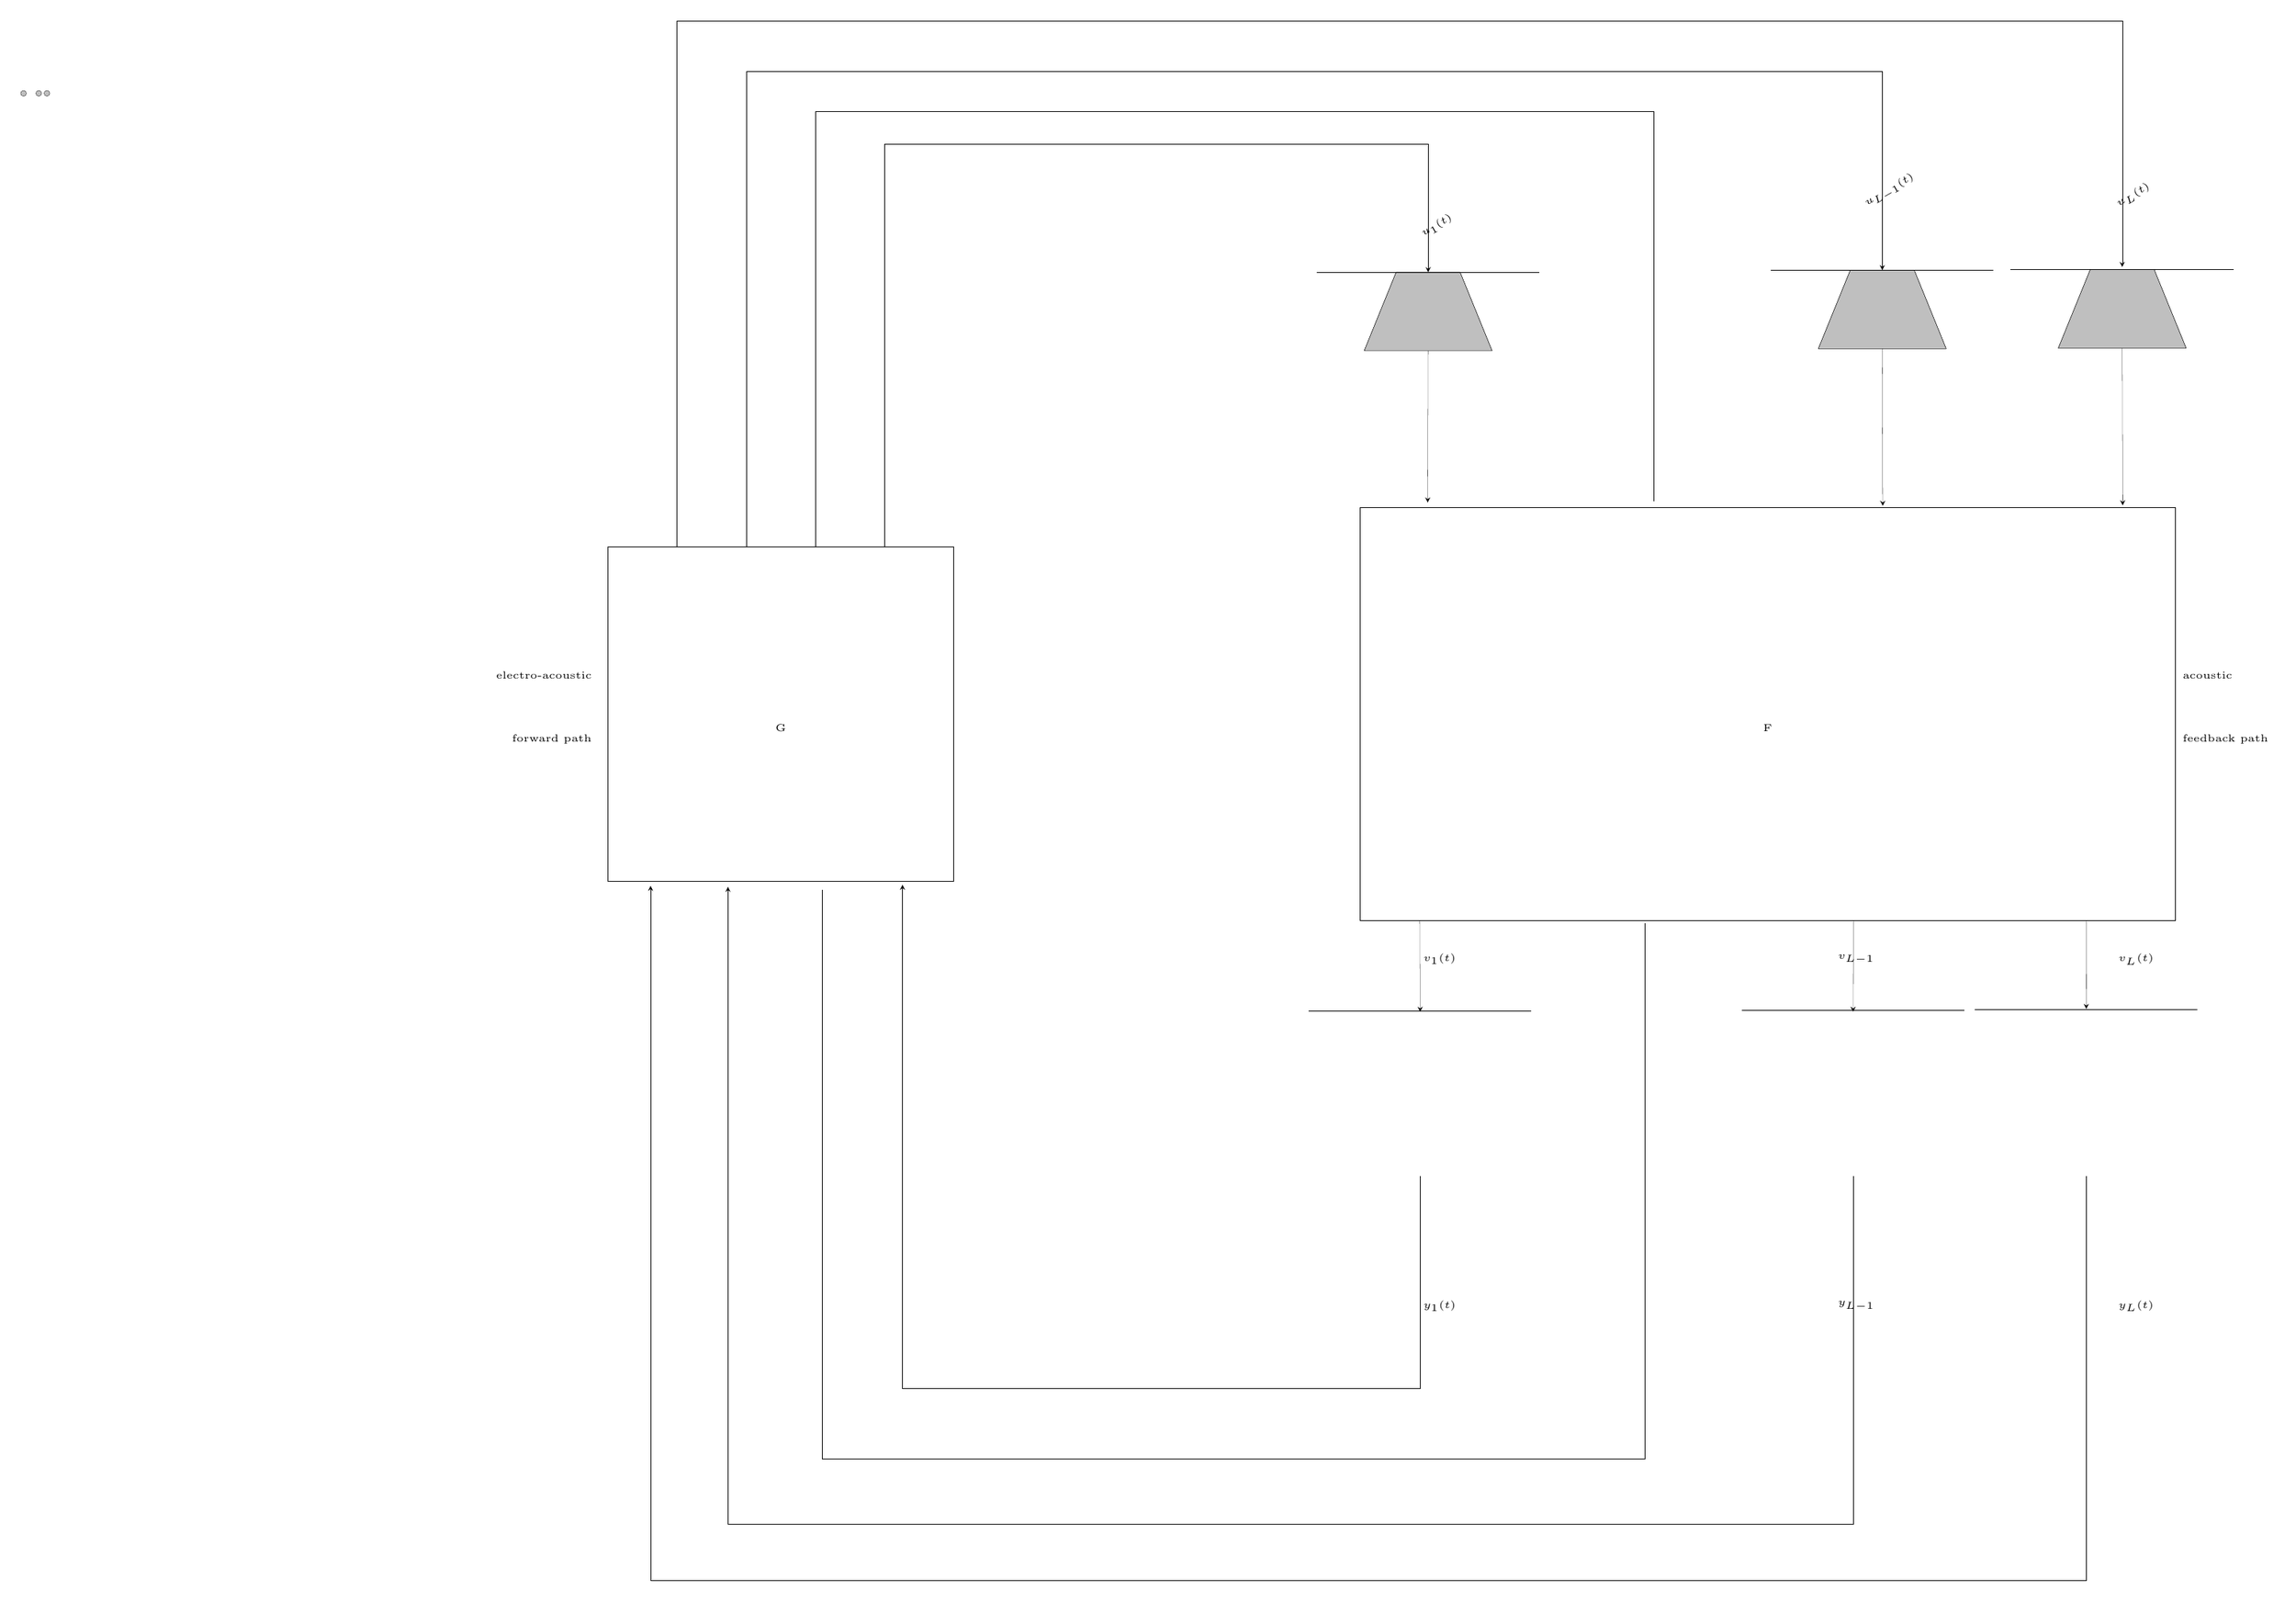
\begin{tikzpicture}
 \tikzstyle{every node}=[font=\tiny]
\pgftransformxscale{1.000000}
\pgftransformyscale{-1.000000}
\definecolor{dialinecolor}{rgb}{0.000000, 0.000000, 0.000000}
\pgfsetstrokecolor{dialinecolor}
\definecolor{dialinecolor}{rgb}{1.000000, 1.000000, 1.000000}
\pgfsetfillcolor{dialinecolor}
\pgfsetlinewidth{0.100000\du}
\pgfsetdash{}{0pt}
\pgfsetdash{}{0pt}
\pgfsetmiterjoin
\definecolor{dialinecolor}{rgb}{1.000000, 1.000000, 1.000000}
\pgfsetfillcolor{dialinecolor}
\fill (10.873900\du,8.392380\du)--(10.873900\du,14.113755\du)--(16.795057\du,14.113755\du)--(16.795057\du,8.392380\du)--cycle;
\definecolor{dialinecolor}{rgb}{0.000000, 0.000000, 0.000000}
\pgfsetstrokecolor{dialinecolor}
\draw (10.873900\du,8.392380\du)--(10.873900\du,14.113755\du)--(16.795057\du,14.113755\du)--(16.795057\du,8.392380\du)--cycle;
% setfont left to latex
\definecolor{dialinecolor}{rgb}{0.000000, 0.000000, 0.000000}
\pgfsetstrokecolor{dialinecolor}
\node at (13.834400\du,11.496850\du){G};
\pgfsetlinewidth{0.100000\du}
\pgfsetdash{}{0pt}
\pgfsetdash{}{0pt}
\pgfsetmiterjoin
\definecolor{dialinecolor}{rgb}{1.000000, 1.000000, 1.000000}
\pgfsetfillcolor{dialinecolor}
\fill (23.753300\du,7.715000\du)--(23.753300\du,14.791145\du)--(37.706643\du,14.791145\du)--(37.706643\du,7.715000\du)--cycle;
\definecolor{dialinecolor}{rgb}{0.000000, 0.000000, 0.000000}
\pgfsetstrokecolor{dialinecolor}
\draw (23.753300\du,7.715000\du)--(23.753300\du,14.791145\du)--(37.706643\du,14.791145\du)--(37.706643\du,7.715000\du)--cycle;
% setfont left to latex
\definecolor{dialinecolor}{rgb}{0.000000, 0.000000, 0.000000}
\pgfsetstrokecolor{dialinecolor}
\node at (30.730000\du,11.498100\du){F};
\pgfsetlinewidth{0.100000\du}
\pgfsetdash{}{0pt}
\pgfsetdash{}{0pt}
\pgfsetmiterjoin
\pgfsetbuttcap
{
\definecolor{dialinecolor}{rgb}{0.000000, 0.000000, 0.000000}
\pgfsetfillcolor{dialinecolor}
% was here!!!
\pgfsetarrowsend{stealth}
{\pgfsetcornersarced{\pgfpoint{0.000000\du}{0.000000\du}}\definecolor{dialinecolor}{rgb}{0.000000, 0.000000, 0.000000}
\pgfsetstrokecolor{dialinecolor}
\draw (12.058100\du,8.392380\du)--(12.058100\du,-0.621502\du)--(36.799274\du,-0.621502\du)--(36.799270\du,3.596142\du);
}}
\pgfsetlinewidth{0.100000\du}
\pgfsetdash{}{0pt}
\pgfsetdash{}{0pt}
\pgfsetbuttcap
{
\definecolor{dialinecolor}{rgb}{0.000000, 0.000000, 0.000000}
\pgfsetfillcolor{dialinecolor}
% was here!!!
\pgfsetarrowsend{stealth}
\definecolor{dialinecolor}{rgb}{0.000000, 0.000000, 0.000000}
\pgfsetstrokecolor{dialinecolor}
\draw (36.799300\du,4.987210\du)--(36.807600\du,7.678280\du);
}
\pgfsetlinewidth{0.100000\du}
\pgfsetdash{}{0pt}
\pgfsetdash{}{0pt}
\pgfsetbuttcap
\pgfsetmiterjoin
\pgfsetlinewidth{0.100000\du}
\pgfsetbuttcap
\pgfsetmiterjoin
\pgfsetdash{}{0pt}
\definecolor{dialinecolor}{rgb}{0.749020, 0.749020, 0.749020}
\pgfsetfillcolor{dialinecolor}
\fill (36.252085\du,3.641490\du)--(37.346454\du,3.641490\du)--(37.893638\du,4.987203\du)--(35.704900\du,4.987203\du)--cycle;
\definecolor{dialinecolor}{rgb}{0.000000, 0.000000, 0.000000}
\pgfsetstrokecolor{dialinecolor}
\draw (36.252085\du,3.641490\du)--(37.346454\du,3.641490\du)--(37.893638\du,4.987203\du)--(35.704900\du,4.987203\du)--cycle;
\pgfsetbuttcap
\pgfsetmiterjoin
\pgfsetdash{}{0pt}
\definecolor{dialinecolor}{rgb}{0.000000, 0.000000, 0.000000}
\pgfsetstrokecolor{dialinecolor}
\draw (36.252085\du,3.641490\du)--(37.346454\du,3.641490\du)--(37.893638\du,4.987203\du)--(35.704900\du,4.987203\du)--cycle;
\pgfsetlinewidth{0.100000\du}
\pgfsetdash{}{0pt}
\pgfsetdash{}{0pt}
\pgfsetbuttcap
{
\definecolor{dialinecolor}{rgb}{0.000000, 0.000000, 0.000000}
\pgfsetfillcolor{dialinecolor}
% was here!!!
\definecolor{dialinecolor}{rgb}{0.000000, 0.000000, 0.000000}
\pgfsetstrokecolor{dialinecolor}
\draw (34.888300\du,3.640380\du)--(38.704200\du,3.640380\du);
}
\pgfsetlinewidth{0.100000\du}
\pgfsetdash{}{0pt}
\pgfsetdash{}{0pt}
\pgfsetbuttcap
{
\definecolor{dialinecolor}{rgb}{0.000000, 0.000000, 0.000000}
\pgfsetfillcolor{dialinecolor}
% was here!!!
\definecolor{dialinecolor}{rgb}{0.000000, 0.000000, 0.000000}
\pgfsetstrokecolor{dialinecolor}
\draw (10.873900\du,8.392380\du)--(16.795000\du,8.392380\du);
}
\pgfsetlinewidth{0.100000\du}
\pgfsetdash{}{0pt}
\pgfsetdash{}{0pt}
\pgfsetmiterjoin
\pgfsetbuttcap
{
\definecolor{dialinecolor}{rgb}{0.000000, 0.000000, 0.000000}
\pgfsetfillcolor{dialinecolor}
% was here!!!
\pgfsetarrowsend{stealth}
{\pgfsetcornersarced{\pgfpoint{0.000000\du}{0.000000\du}}\definecolor{dialinecolor}{rgb}{0.000000, 0.000000, 0.000000}
\pgfsetstrokecolor{dialinecolor}
\draw (15.610800\du,8.392380\du)--(15.610800\du,1.487530\du)--(24.917000\du,1.487530\du)--(24.917000\du,3.686090\du);
}}
\pgfsetlinewidth{0.100000\du}
\pgfsetdash{}{0pt}
\pgfsetdash{}{0pt}
\pgfsetbuttcap
{
\definecolor{dialinecolor}{rgb}{0.000000, 0.000000, 0.000000}
\pgfsetfillcolor{dialinecolor}
% was here!!!
\pgfsetarrowsend{stealth}
\definecolor{dialinecolor}{rgb}{0.000000, 0.000000, 0.000000}
\pgfsetstrokecolor{dialinecolor}
\draw (24.917000\du,5.031800\du)--(24.909100\du,7.629670\du);
}
\pgfsetlinewidth{0.100000\du}
\pgfsetdash{}{0pt}
\pgfsetdash{}{0pt}
\pgfsetmiterjoin
\pgfsetbuttcap
{
\definecolor{dialinecolor}{rgb}{0.000000, 0.000000, 0.000000}
\pgfsetfillcolor{dialinecolor}
% was here!!!
\pgfsetarrowsend{stealth}
{\pgfsetcornersarced{\pgfpoint{0.000000\du}{0.000000\du}}\definecolor{dialinecolor}{rgb}{0.000000, 0.000000, 0.000000}
\pgfsetstrokecolor{dialinecolor}
\draw (13.242300\du,8.392380\du)--(13.242300\du,0.250649\du)--(32.691300\du,0.250649\du)--(32.691300\du,3.650940\du);
}}
\pgfsetlinewidth{0.100000\du}
\pgfsetdash{}{0pt}
\pgfsetdash{}{0pt}
\pgfsetbuttcap
{
\definecolor{dialinecolor}{rgb}{0.000000, 0.000000, 0.000000}
\pgfsetfillcolor{dialinecolor}
% was here!!!
\pgfsetarrowsend{stealth}
\definecolor{dialinecolor}{rgb}{0.000000, 0.000000, 0.000000}
\pgfsetstrokecolor{dialinecolor}
\draw (32.691300\du,4.996650\du)--(32.699600\du,7.687730\du);
}
\pgfsetlinewidth{0.100000\du}
\pgfsetdash{}{0pt}
\pgfsetdash{}{0pt}
\pgfsetbuttcap
\pgfsetmiterjoin
\pgfsetlinewidth{0.100000\du}
\pgfsetbuttcap
\pgfsetmiterjoin
\pgfsetdash{}{0pt}
\definecolor{dialinecolor}{rgb}{0.749020, 0.749020, 0.749020}
\pgfsetfillcolor{dialinecolor}
\fill (32.144185\du,3.650940\du)--(33.238554\du,3.650940\du)--(33.785738\du,4.996653\du)--(31.597000\du,4.996653\du)--cycle;
\definecolor{dialinecolor}{rgb}{0.000000, 0.000000, 0.000000}
\pgfsetstrokecolor{dialinecolor}
\draw (32.144185\du,3.650940\du)--(33.238554\du,3.650940\du)--(33.785738\du,4.996653\du)--(31.597000\du,4.996653\du)--cycle;
\pgfsetbuttcap
\pgfsetmiterjoin
\pgfsetdash{}{0pt}
\definecolor{dialinecolor}{rgb}{0.000000, 0.000000, 0.000000}
\pgfsetstrokecolor{dialinecolor}
\draw (32.144185\du,3.650940\du)--(33.238554\du,3.650940\du)--(33.785738\du,4.996653\du)--(31.597000\du,4.996653\du)--cycle;
\pgfsetlinewidth{0.100000\du}
\pgfsetdash{}{0pt}
\pgfsetdash{}{0pt}
\pgfsetbuttcap
{
\definecolor{dialinecolor}{rgb}{0.000000, 0.000000, 0.000000}
\pgfsetfillcolor{dialinecolor}
% was here!!!
\definecolor{dialinecolor}{rgb}{0.000000, 0.000000, 0.000000}
\pgfsetstrokecolor{dialinecolor}
\draw (30.780300\du,3.649820\du)--(34.596200\du,3.649820\du);
}
\pgfsetlinewidth{0.100000\du}
\pgfsetdash{{\pgflinewidth}{0.200000\du}}{0cm}
\pgfsetdash{{\pgflinewidth}{0.200000\du}}{0cm}
\pgfsetmiterjoin
\pgfsetbuttcap
{
\definecolor{dialinecolor}{rgb}{0.000000, 0.000000, 0.000000}
\pgfsetfillcolor{dialinecolor}
% was here!!!
{\pgfsetcornersarced{\pgfpoint{0.000000\du}{0.000000\du}}\definecolor{dialinecolor}{rgb}{0.000000, 0.000000, 0.000000}
\pgfsetstrokecolor{dialinecolor}
\draw (14.426600\du,8.392380\du)--(14.426600\du,0.934434\du)--(28.777600\du,0.934434\du)--(28.777600\du,7.593900\du);
}}
\pgfsetlinewidth{0.100000\du}
\pgfsetdash{}{0pt}
\pgfsetdash{}{0pt}
\pgfsetbuttcap
{
\definecolor{dialinecolor}{rgb}{0.000000, 0.000000, 0.000000}
\pgfsetfillcolor{dialinecolor}
% was here!!!
\pgfsetarrowsend{stealth}
\definecolor{dialinecolor}{rgb}{0.000000, 0.000000, 0.000000}
\pgfsetstrokecolor{dialinecolor}
\draw (36.186300\du,14.800800\du)--(36.184300\du,16.303500\du);
}
\pgfsetlinewidth{0.100000\du}
\pgfsetdash{}{0pt}
\pgfsetdash{}{0pt}
\pgfsetbuttcap
{
\definecolor{dialinecolor}{rgb}{0.000000, 0.000000, 0.000000}
\pgfsetfillcolor{dialinecolor}
% was here!!!
\pgfsetarrowsend{stealth}
\definecolor{dialinecolor}{rgb}{0.000000, 0.000000, 0.000000}
\pgfsetstrokecolor{dialinecolor}
\draw (24.774100\du,14.800800\du)--(24.780500\du,16.352900\du);
}
\pgfsetlinewidth{0.100000\du}
\pgfsetdash{}{0pt}
\pgfsetdash{}{0pt}
\pgfsetbuttcap
{
\definecolor{dialinecolor}{rgb}{0.000000, 0.000000, 0.000000}
\pgfsetfillcolor{dialinecolor}
% was here!!!
\pgfsetarrowsend{stealth}
\definecolor{dialinecolor}{rgb}{0.000000, 0.000000, 0.000000}
\pgfsetstrokecolor{dialinecolor}
\draw (32.195900\du,14.800800\du)--(32.192900\du,16.352900\du);
}
\pgfsetlinewidth{0.100000\du}
\pgfsetdash{{\pgflinewidth}{0.200000\du}}{0cm}
\pgfsetdash{{\pgflinewidth}{0.200000\du}}{0cm}
\pgfsetmiterjoin
\pgfsetbuttcap
{
\definecolor{dialinecolor}{rgb}{0.000000, 0.000000, 0.000000}
\pgfsetfillcolor{dialinecolor}
% was here!!!
{\pgfsetcornersarced{\pgfpoint{0.000000\du}{0.000000\du}}\definecolor{dialinecolor}{rgb}{0.000000, 0.000000, 0.000000}
\pgfsetstrokecolor{dialinecolor}
\draw (28.630000\du,14.841600\du)--(28.630000\du,24.006200\du)--(14.546000\du,24.006200\du)--(14.546000\du,14.256400\du);
}}
\pgfsetlinewidth{0.100000\du}
\pgfsetdash{}{0pt}
\pgfsetdash{}{0pt}
\pgfsetmiterjoin
\pgfsetbuttcap
{
\definecolor{dialinecolor}{rgb}{0.000000, 0.000000, 0.000000}
\pgfsetfillcolor{dialinecolor}
% was here!!!
\pgfsetarrowsend{stealth}
{\pgfsetcornersarced{\pgfpoint{0.000000\du}{0.000000\du}}\definecolor{dialinecolor}{rgb}{0.000000, 0.000000, 0.000000}
\pgfsetstrokecolor{dialinecolor}
\draw (32.192900\du,19.169900\du)--(32.192900\du,25.130100\du)--(12.931200\du,25.130100\du)--(12.931200\du,14.214400\du);
}}
\pgfsetlinewidth{0.100000\du}
\pgfsetdash{}{0pt}
\pgfsetdash{}{0pt}
\pgfsetmiterjoin
\pgfsetbuttcap
{
\definecolor{dialinecolor}{rgb}{0.000000, 0.000000, 0.000000}
\pgfsetfillcolor{dialinecolor}
% was here!!!
\pgfsetarrowsend{stealth}
{\pgfsetcornersarced{\pgfpoint{0.000000\du}{0.000000\du}}\definecolor{dialinecolor}{rgb}{0.000000, 0.000000, 0.000000}
\pgfsetstrokecolor{dialinecolor}
\draw (36.182400\du,19.169900\du)--(36.182400\du,26.084700\du)--(11.605400\du,26.084700\du)--(11.605400\du,14.196700\du);
}}
\pgfsetlinewidth{0.100000\du}
\pgfsetdash{}{0pt}
\pgfsetdash{}{0pt}
\pgfsetmiterjoin
\pgfsetbuttcap
{
\definecolor{dialinecolor}{rgb}{0.000000, 0.000000, 0.000000}
\pgfsetfillcolor{dialinecolor}
% was here!!!
\pgfsetarrowsend{stealth}
{\pgfsetcornersarced{\pgfpoint{0.000000\du}{0.000000\du}}\definecolor{dialinecolor}{rgb}{0.000000, 0.000000, 0.000000}
\pgfsetstrokecolor{dialinecolor}
\draw (24.780500\du,19.169900\du)--(24.780500\du,22.806200\du)--(15.918700\du,22.806200\du)--(15.918700\du,14.179000\du);
}}
% setfont left to latex
\definecolor{dialinecolor}{rgb}{0.000000, 0.000000, 0.000000}
\pgfsetstrokecolor{dialinecolor}
\node[anchor=west,rotate=30] at (24.716400\du,3.093200\du){$u_1(t)$};
\node[anchor=west,rotate=30] at (32.316400\du,2.593200\du){$u_{L-1}(t)$};
\node[anchor=west,rotate=30] at (36.616400\du,2.593200\du){$u_{L}(t)$};

\node[anchor=west] at (24.716400\du,15.453200\du){$v_1(t)$};
\node[anchor=west] at (31.816400\du,15.453200\du){$v_{L-1}$};
\node[anchor=west] at (36.616400\du,15.453200\du){$v_{L}(t)$};

\node[anchor=east] at (10.716400\du,10.593200\du){electro-acoustic};
\node[anchor=east] at (10.716400\du,11.693200\du){forward path};

\node[anchor=west] at (37.716400\du,10.593200\du){acoustic};
\node[anchor=west] at (37.716400\du,11.693200\du){feedback path};

% setfont left to latex
\definecolor{dialinecolor}{rgb}{0.000000, 0.000000, 0.000000}
\pgfsetstrokecolor{dialinecolor}
\node[anchor=west] at (24.716400\du,21.393200\du){$y_1(t)$};
\node[anchor=west] at (31.816400\du,21.393200\du){$y_{L-1}$};
\node[anchor=west] at (36.616400\du,21.393200\du){$y_{L}(t)$};
\pgfsetlinewidth{0.100000\du}
\pgfsetdash{}{0pt}
\pgfsetdash{}{0pt}
\pgfsetbuttcap
\pgfsetmiterjoin
\pgfsetlinewidth{0.100000\du}
\pgfsetbuttcap
\pgfsetmiterjoin
\pgfsetdash{}{0pt}
\definecolor{dialinecolor}{rgb}{0.749020, 0.749020, 0.749020}
\pgfsetfillcolor{dialinecolor}
\fill (24.369785\du,3.686090\du)--(25.464154\du,3.686090\du)--(26.011338\du,5.031803\du)--(23.822600\du,5.031803\du)--cycle;
\definecolor{dialinecolor}{rgb}{0.000000, 0.000000, 0.000000}
\pgfsetstrokecolor{dialinecolor}
\draw (24.369785\du,3.686090\du)--(25.464154\du,3.686090\du)--(26.011338\du,5.031803\du)--(23.822600\du,5.031803\du)--cycle;
\pgfsetbuttcap
\pgfsetmiterjoin
\pgfsetdash{}{0pt}
\definecolor{dialinecolor}{rgb}{0.000000, 0.000000, 0.000000}
\pgfsetstrokecolor{dialinecolor}
\draw (24.369785\du,3.686090\du)--(25.464154\du,3.686090\du)--(26.011338\du,5.031803\du)--(23.822600\du,5.031803\du)--cycle;
\pgfsetlinewidth{0.100000\du}
\pgfsetdash{}{0pt}
\pgfsetdash{}{0pt}
\pgfsetbuttcap
{
\definecolor{dialinecolor}{rgb}{0.000000, 0.000000, 0.000000}
\pgfsetfillcolor{dialinecolor}
% was here!!!
\definecolor{dialinecolor}{rgb}{0.000000, 0.000000, 0.000000}
\pgfsetstrokecolor{dialinecolor}
\draw (23.005900\du,3.684970\du)--(26.821900\du,3.684970\du);
}
\definecolor{dialinecolor}{rgb}{0.749020, 0.749020, 0.749020}
\pgfsetfillcolor{dialinecolor}
\pgfpathellipse{\pgfpoint{24.780481\du}{17.761381\du}}{\pgfpoint{1.408481\du}{0\du}}{\pgfpoint{0\du}{1.408481\du}}
\pgfusepath{fill}
\pgfsetlinewidth{0.100000\du}
\pgfsetdash{}{0pt}
\pgfsetdash{}{0pt}
\definecolor{dialinecolor}{rgb}{0.000000, 0.000000, 0.000000}
\pgfsetstrokecolor{dialinecolor}
\pgfpathellipse{\pgfpoint{24.780481\du}{17.761381\du}}{\pgfpoint{1.408481\du}{0\du}}{\pgfpoint{0\du}{1.408481\du}}
\pgfusepath{stroke}
\pgfsetlinewidth{0.100000\du}
\pgfsetdash{}{0pt}
\pgfsetdash{}{0pt}
\pgfsetbuttcap
{
\definecolor{dialinecolor}{rgb}{0.000000, 0.000000, 0.000000}
\pgfsetfillcolor{dialinecolor}
% was here!!!
\definecolor{dialinecolor}{rgb}{0.000000, 0.000000, 0.000000}
\pgfsetstrokecolor{dialinecolor}
\draw (22.864400\du,16.340900\du)--(26.680300\du,16.340900\du);
}
\definecolor{dialinecolor}{rgb}{0.749020, 0.749020, 0.749020}
\pgfsetfillcolor{dialinecolor}
\pgfpathellipse{\pgfpoint{32.202681\du}{17.738581\du}}{\pgfpoint{1.408481\du}{0\du}}{\pgfpoint{0\du}{1.408481\du}}
\pgfusepath{fill}
\pgfsetlinewidth{0.100000\du}
\pgfsetdash{}{0pt}
\pgfsetdash{}{0pt}
\definecolor{dialinecolor}{rgb}{0.000000, 0.000000, 0.000000}
\pgfsetstrokecolor{dialinecolor}
\pgfpathellipse{\pgfpoint{32.202681\du}{17.738581\du}}{\pgfpoint{1.408481\du}{0\du}}{\pgfpoint{0\du}{1.408481\du}}
\pgfusepath{stroke}
\pgfsetlinewidth{0.100000\du}
\pgfsetdash{}{0pt}
\pgfsetdash{}{0pt}
\pgfsetbuttcap
{
\definecolor{dialinecolor}{rgb}{0.000000, 0.000000, 0.000000}
\pgfsetfillcolor{dialinecolor}
% was here!!!
\definecolor{dialinecolor}{rgb}{0.000000, 0.000000, 0.000000}
\pgfsetstrokecolor{dialinecolor}
\draw (30.286600\du,16.318000\du)--(34.102500\du,16.318000\du);
}
\definecolor{dialinecolor}{rgb}{0.749020, 0.749020, 0.749020}
\pgfsetfillcolor{dialinecolor}
\pgfpathellipse{\pgfpoint{36.186481\du}{17.734181\du}}{\pgfpoint{1.408481\du}{0\du}}{\pgfpoint{0\du}{1.408481\du}}
\pgfusepath{fill}
\pgfsetlinewidth{0.100000\du}
\pgfsetdash{}{0pt}
\pgfsetdash{}{0pt}
\definecolor{dialinecolor}{rgb}{0.000000, 0.000000, 0.000000}
\pgfsetstrokecolor{dialinecolor}
\pgfpathellipse{\pgfpoint{36.186481\du}{17.734181\du}}{\pgfpoint{1.408481\du}{0\du}}{\pgfpoint{0\du}{1.408481\du}}
\pgfusepath{stroke}
\pgfsetlinewidth{0.100000\du}
\pgfsetdash{}{0pt}
\pgfsetdash{}{0pt}
\pgfsetbuttcap
{
\definecolor{dialinecolor}{rgb}{0.000000, 0.000000, 0.000000}
\pgfsetfillcolor{dialinecolor}
% was here!!!
\definecolor{dialinecolor}{rgb}{0.000000, 0.000000, 0.000000}
\pgfsetstrokecolor{dialinecolor}
\draw (34.270400\du,16.313600\du)--(38.086300\du,16.313600\du);
}
\end{tikzpicture}

    \end{center}
    \caption{Discrete-time model of a Sound reinforcement system}
    \label{feedmodel}
\end{figure} 
Mathematically this can be represented as:
\begin{eqnarray}
\mathbf{y}= \mathbf{F}(q,t)\mathbf{u}(t) + \mathbf{v}(t)\\
\mathbf{u} = \mathbf{G}[\mathbf{y}(t),t]
\end{eqnarray}
The source signal $\mathbf{v}_i(t)$, microphone signal $\mathbf{y}_i(t)$ and loudspeaker signal vectors $\mathbf{u}_j(t)$ are defined as: 
\begin{eqnarray}
\mathbf{v}(t) = [v_1(t) \ldots v_S]^T \\
\mathbf{y}(t) = [y_1(t) \ldots y_S]^T \\
\mathbf{u}(t) = [u_1(t) \ldots v_L]^T
\end{eqnarray}
The matrix $\mathbf{F}(q,t)$ is the multi channel acoustic \textit{feedback path}, $\mathbf{G}(\cdot,t)$ is the electroacoustic forward path characteristics or \textit{forward path}.

Between each loudspeaker-microphone pair $(i,j)$ there exists an acoustic coupling, this is modeled by the nth order acoustic feedback path transfer function:
\begin{equation}
	F_{ij}(q,t) = f_{ij}^{(0)}(t) + f_{ij}^{(1)}(t)q^{-1} + \ldots + f_{ij}^{(n_F)}(t)q^{-n_F}
\end{equation}
$q$ is the discrete time shift operator: $q^{-k}f(t) = f(t-k)$.

We can define the feedback path as a matrix of all the possible couplings:
\begin{eqnarray}
\mathbf{F}(q,t) =
\begin{bmatrix}
F_{11}(q,t) & \ldots & F_{1L}(q,t)\\
\vdots & \ldots & \vdots\\
F_{S1}(q,t) & \ldots & F_{SL}(q,t)
\end{bmatrix}
\end{eqnarray}
The acoustic feedback path model is linear, time varying and of finite order \cite{van_waterschoot_fifty_2011}.\\

The proposed solution simplifies this path by assuming a single speaker a single microphone, this is not a unreasonable assumption since most sound reinforcement systems for speech consists of two speakers and one microphone. The simplified version of the feedback path seems good enough to provide a proof of concept. The resulting model for both the feedback and feed-forward path can be seen as scalar.\\

\subsection{Two-stage NHS}
\index{Notch-filter}
\nomenclature{NHS}{Notch filter Howling Suppression} 
The method used in this system is the two-stage Notch filter based Howling Suppression (NHS), this is a simple and reliable method that is commonly used in howling prevention \cite{van_waterschoot_fifty_2011}. The figure \ref{NHS_overview} shows the overall conceptual structure of the method.

\begin{figure}[H]
\centering
\includegraphics[width=14cm]{description/Figures/Two-stage_NHS-2}
\caption{Two-stage NHS structure}
\label{NHS_overview}
\end{figure}

In this figure \ref{NHS_overview} $G$ is the transfer function of the electro-acoustical feed forward path, $F$ is the feedback path, and $H$ is an equalizer that consists of a bank of adjustable notch-filters. The signals are given by non-capital letters where $v(t)$ is the wanted audio signal from the person or instrument in front of the microphone, $y(t)$ is one frame of samples of this signal in the time plane, $D$ is a vector of frequencies where howling has been detected, $d(t)$ is the signal after it has been filtered though the adjustable bank of notch-filters, $u(t)$ is the output to the speaker(s), $x(t)$ is the unwanted feedback signal.\\
\\
\index{howling}\index{feedback loop}
The howling detection is designed to detect howling and return a vector of frequencies on which howling is detected. These frequencies will correspond to a notch-filter in the equalizer, reducing the gain on these frequencies. Hopefully this reduction in frequency gain is enough to break the positive feedback loop end stop the howling. \\
\\
\index{power spectrum}
The howling detection scheme looks at the power spectrum of the signal and picks out peaks, these peaks are subjected to several tests. Peaks are tested for discriminating features between howling and a normal sinusoidal tone, since most tones have harmonic components the frequencies that have harmonics can be eliminated as a candidate for howling. The signals where no harmonics are detected is tested by looking at the following parameters:\\
\begin{itemize}
\index{PTPR}\index{PAPR}\index{PNPR}\index{IPMP}\index{PHPR}\index{IMSD}
\item Peak-to-threshold power ratio(PTPR)\nomenclature{PTPR}{Peak-to-threshold power ratio} 
\subitem between the peak magnitude and predefined constant magnitude
\item Peak-to-average power ratio(PAPR)\nomenclature{PAPR}{Peak-to-average power ratio} 
\subitem The ratio between the peak magnitude and the average of the signal
\item Peak-to-neighboring power ratio(PNPR)\nomenclature{PNPR}{Peak-to-neighboring power ratio} 
\subitem The ratio between the peak magnitude and other nearby peaks
\item Interframe peak magnitude persistence (IPMP)\nomenclature{IPMP}{Interframe peak magnitude persistence}
\subitem How persistent this peak is in a sample of previous frames

\item Peak-to-harmonic peak ratio(PHPR)\nomenclature{PHPR}{Peak-to-harmonic peak ratio}
\subitem The ratio between the peak magnitude and the magnitude of its first harmonic peak
\item Interframe magnitude slope deviation (IMSD)\nomenclature{IMSD}{Interframe magnitude slope deviation}
\subitem How the magnitude of this peak is changing over the previous frames
\end{itemize}
\index{howling}
Based on these parameters or a subset of these parameters a state of howling can be detected. The different ratios must be tuned to give good performance.




\section{Implementation}

\begin{figure}
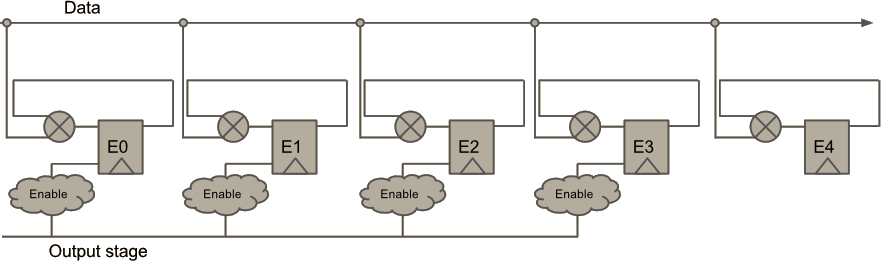
\includegraphics[width=15cm]{implementation/fig_ecc}
\caption{Implementation of Hamming(16,11)}
\label{fig:ecc}
\end{figure}

\section{Tests}
\subsection{Overview}
The liaison system was verified utilizing automated testbenches. The testbenches uses VHDL assertions to notify the author if any
of the tests failed. In order to create a good and short but extensive testbench, we have built a collection of procedures that takes input, expected output
and expected system status after all input has been sent.

The test cases was divided into three blocks.
\begin{itemize}
\item The first test block consists of 8 tests that asserts the normal behaviour. It is done with some easy cases and a 2 cycle delay between inputs.

\item The second test block consists of 24 cases that at some point broke our logic.  tests where our design was likly to have flaws. During development, these tests were
triggered often, proving their value.

\item The third and last test block is a permutation of working state and all 4! fail states, each with all MCUs sending
all possible inputs (all MCUs sends the same value to keep the number of tests down to an affordable number). This block consists of 269 376 different test cases,
and cover almost any possible state. The states that are not covered are those where one of the MCUs fails in the middle of the transaction, which are covered in
the second block.
\end{itemize}

Since all permutations of fail states and all permutations of valid input within these states
were applied to the circuit during simulation, we are confident that the Liaison System is working correctly. We have also tested the circuit with a post-place and route
simulation verifying that the output is also correct with timing taken into account\footnote{The timing simulation was done with iSim from Xilinx, synthesised with XST. Both tools are part of the ISE Design Suite}.

\subsection{Conformance with requirements specification}
This section explain the conformance with each point in the system requirements specification.
\begin{enumerate}
\item{\textbf{The Liaison Interface}} \hfill\\
    Our implementation of the Liaison System follows the signaling interface given by the requirements\cite{task}.

\item{\textbf{Voting}} \hfill\\
    The Voting algorithm has been tested and confirmed to be working. This was done by enumerating all
    permutations of input and state, and then check the Voters result against expected output using
    VHDL assertions.

\item{\textbf{Error tagging}} \hfill\\
    The error tagging is not specified in the requirements, but is nessesary in our implementation to
    achieve correct System Status bits and correct Voting. The error tagging was tested with the same
    tests as the Voting algorithm and does conform with the expected behaviour.

\item{\textbf{System status}} \hfill\\
    The System Status is needed to tell the receiver about the wellness of the microcontrollers. Since
    there exists a direct mapping between the Error tagging and the System Status, this is also
    included in the same tests as Error tagging and Voting.

\item{\textbf{Error correcting code}} \hfill\\
    The Error correcting code is a specific part of the requirements\cite{task}. The module was tested by writing
    a testbench function that generates (15,11)-Hamming Code with SECDED from an 11-bit word. This
    procedure was added to the enumerated tests from the Voter-test such that for each input, the testbench
    would automatically expect a specific ECC. If the ECC from the function was not equal to the output
    of the Liaison, assertions were raised to the tester. Since the soft function agrees with the simulated
    hardware, we are certain that the ECC-module works as specified in the requirements. The ECC-generating
    software function can be found in \autoref{apx:ecc}.

\item{\textbf{Reset behaviour}} \hfill\\
    On reset, The Liaison is set back to inital state on next clock cycle. The reset is stricly synchronous,
    as stated in the requirements\cite{task}, and is thus only read on rising edge of the clock. We have
    tested that reset works for any final state when a data sequence finished, but we have not tested the
    behavoiur of a reset in the middle of a transmission. By simple code inspection, we see that the
    reset is not aware of current system status, but simply sets all the state variables back to initial
    state. That means that after a reset signal is asserted along with rising edge of the clock, the system
    will not process data until a new {\ttfamily di\_ready}.

\item{\textbf{System consitency}} \hfill\\
    Since all possible inputs for both the Voter and the ECC module has been exhaustively tested, and 
    Since very little of the internal system logic is dependent on both system status and current bit-position,
    we are sure that the exhaustive tests run on the Voter and the ECC module is sufficient to conclude that 
    the entire system is consitent with the requirements. All enumerations of fail states have been tested, all combinations
    of input to the ECC module have been tested, and the Output Multiplexer cares only about current output bit position,
    and is thus also exhaustivly tested.

\item{\textbf{New data after $11+m$ cycles}} \hfill\\
    Most of the test cases send data directly after previous data word was correctly received, so 
    Our implementation of the Liaison System follows the signaling interface given by the requirements.

\end{enumerate}

\todo{Include timing diagrams}
\section{Conclusion}
\section{Conclusion}
From testing and verifying software prototype this report displays a working proof of concept of a feedback cancellation  algorithm based on the two-stage NHS method. The front end interface and output interface has been constructed and tested. All has been verified to work according to specifications.

\section{Further work}
The NHS algorithm is a simple one, and in this design it is further simplified. There are a number of ratios used in NHS that can be calculated to improve the detection capabilities, examples of these ratios can be found in \cite{van_waterschoot_fifty_2011}. \\

There are also more advanced algorithms for removing feedback, for instance a AFC-method(Adaptive Feedback Cancellation). The AFC uses system identification to detect the feedback path and models its inverse, thereby cancelling the coupling. Details can be found in \cite{van_waterschoot_fifty_2011}.\\

Transforming the system from a software prototype to a hardware prototype can be done by as previously stated using a FPGA as the DSP-module and implementing the algorithm on it.\\
The broader goal is a finished product. Working on product design, a complete hardware design and doing marked research are all important tasks in completing the project.

\appendix
\bibliographystyle{plain}
\bibliography{bibliography}

\end{document}
